\chapter{Specifikacija programske potpore}
		
	\section{Funkcionalni zahtjevi}
			
			\textbf{\textit{dio 1. revizije}}\\
			
			\textit{Navesti \textbf{dionike} koji imaju \textbf{interes u ovom sustavu} ili  \textbf{su nositelji odgovornosti}. To su prije svega korisnici, ali i administratori sustava, naručitelji, razvojni tim.}\\
				
			\textit{Navesti \textbf{aktore} koji izravno \textbf{koriste} ili \textbf{komuniciraju sa sustavom}. Oni mogu imati inicijatorsku ulogu, tj. započinju određene procese u sustavu ili samo sudioničku ulogu, tj. obavljaju određeni posao. Za svakog aktora navesti funkcionalne zahtjeve koji se na njega odnose.}\\
			
			
			\noindent \textbf{Dionici:}
			
			\begin{packed_enum}
				\item Naručitelj
				\item Javnost
				\item Korisnici
				\item Organizator
				\item Glazbenik 							
				\item Administrator
				\item Razvojni tim
			\end{packed_enum}
			
\noindent \textbf{Aktori i njihovi funkcionalni zahtjevi:}


\begin{packed_enum}


	\item  \underbar{Neprijavljeni/neregistrirani korisnik (javnost) može:}
				
	\begin{packed_enum}
		\item Pregledati javne događaje
		\item Pregledati profil benda
		\item Vidjeti recenzije
		\item Registrirati se na aplikaciji
	\end{packed_enum}
			
	\item  \underbar{Korisnik (inicijator) može:}
	
	\begin{packed_enum}
		
		\item Sve što i Javnost
		\item Prijaviti se na aplikaciju
		\item Pregledavati i uređivati korisnički profil
		\item Pregledati postoječe poruke s drugim korisnicima
		\item Pregledati svoj kalendar
		\item Slati nove poruke drugim korisnicima
		\item Recenzirati događaje
		\item Komentirati objave glazbenika
		\item Postati glazbenik i/ili organizator
		\item Pisati objave na svom profilu
		\item odjaviti se 
		
	\end{packed_enum}
	
	
	\item  \underbar{Glazbenik (inicijator) može:}
	
	\begin{packed_enum}
		
		\item Sve što i Korisnik
		\item Prihvatiti ili odbiti poziv u bend
		\item Postati članom jednog ili više bendova
		\item Održati samostalan nastup
		\item Stvoriti bend
	\end{packed_enum}
	
	\item  \underbar{Organizator (inicijator) može:}
	
	\begin{packed_enum}
		
		\item Sve što i Korisnik
		\item Pretraživati bendove na aplikaciji
		\item Stvarati događaje
		\item Uređivati događaje
		\item Recenzirati bend kao organizator događaja
	\end{packed_enum}
	
	\item  \underbar{Voditelj benda (inicijator) može:}
	
	\begin{packed_enum}
		
		\item Sve što i Glazbenik
		\item Pozivati i dodavati nove članove u bend
		\item Dodavati obaveze u kalendar benda
		\item Vidjeti kalendare članova benda
		\item Recenzirati organizatora u ime benda
		\item Objavljivate objave na stranici benda
		\item Uređivati profil benda
	\end{packed_enum}
	
	\item  \underbar{Administrator (inicijator) može:}
	
	\begin{packed_enum}
		
		\item Blokirati korisnike koji su prekršili uvjete korištenja aplikacije
		\item Uređivati popis instrumenata
		\item Dodavati događaje koji su stvoreni na drugim platformama
		
	\end{packed_enum}
	
	\item  \underbar{Baza podataka (sudionik) može:}
	
	\begin{packed_enum}
		
		\item Pohranjuje sve podatke o korisnicima, glazbenicima, organizatorima i bendovima
		\item Pohranjuje sve podatke o nastupima, recenzijama, objavama, komentarima
		\item Pohranjuje sve razmijenjene poruke između korisnika 
		
	\end{packed_enum}
		
\end{packed_enum}
			
\eject 
			
			
				
\subsection{Obrasci uporabe}

\textbf{\textit{dio 1. revizije}}

\subsubsection{Opis obrazaca uporabe}
	\textit{Funkcionalne zahtjeve razraditi u obliku obrazaca uporabe. Svaki obrazac je potrebno razraditi prema donjem predlošku. Ukoliko u nekom koraku može doći do odstupanja, potrebno je to odstupanje opisati i po mogućnosti ponuditi rješenje kojim bi se tijek obrasca vratio na osnovni tijek.}\\


\noindent \underbar{\textbf{UC1 - Pristup listi javnih događaja}}
	\begin{packed_item}
		
		\item \textbf{Glavni sudionik: } Javnost
		\item  \textbf{Cilj:} Vidjeti listu javnih događaja na aplikaciji
		\item  \textbf{Sudionici:} Baza podataka
		\item  \textbf{Preduvjet:} -
		\item  \textbf{Prioritet:} High
		\item  \textbf{Opis osnovnog tijeka:}
		
		\item[] \begin{packed_enum}
			\item Javnost na početnoj stranici odabire prikaz događaja
			\item Aplikacija prikazuje javne događaje
		\end{packed_enum}
		
	\end{packed_item}


\noindent \underbar{\textbf{UC2 - Pregled profila benda}}
	\begin{packed_item}
	
		\item \textbf{Glavni sudionik:} Javnost
		\item  \textbf{Cilj:} Vidjeti profil benda
		\item  \textbf{Sudionici:} Baza podataka
		\item  \textbf{Preduvjet:} -
		\item  \textbf{Prioritet:} High
		\item  \textbf{Opis osnovnog tijeka:}
		
		\item[] \begin{packed_enum}
			\item Javnost odabire bend čiji profil želi pregledati
			\item Aplikacija prikazuje profil odabranog benda
		\end{packed_enum}
	
	\end{packed_item}


\noindent \underbar{\textbf{UC3 - Pregled recenzija}}
	\begin{packed_item}
	
		\item \textbf{Glavni sudionik: }Javnost
		\item  \textbf{Cilj:} Vidjeti pregled recenzija
		\item  \textbf{Sudionici:} Baza podataka
		\item  \textbf{Preduvjet:} -
		\item  \textbf{Prioritet:} Medium
		\item  \textbf{Opis osnovnog tijeka:}
		
		\item[] \begin{packed_enum}
			\item Javnost odabire popis recenzija
			\item Aplikacija prikaže popis recenzija
			\item Javnost odabere recenziju koju želi vidjeti
			\item Aplikacija korisniku prikaže odabranu recenziju
		\end{packed_enum}
	\end{packed_item}


\noindent \underbar{\textbf{UC4 - Registracija}}
	\begin{packed_item}
	
		\item \textbf{Glavni sudionik: }Javnost
		\item  \textbf{Cilj:} Registrirati se
		\item  \textbf{Sudionici:} Baza podataka
		\item  \textbf{Preduvjet:} -
		\item  \textbf{Prioritet:} High
		\item  \textbf{Opis osnovnog tijeka:}
		
		\item[] \begin{packed_enum}

			\item Javnost odabire opciju za registraciju
			\item Aplikacija korisniku daje formu za registraciju
			\item Javnost unosi tražene korisničke podatke
			\item Aplikacije korisniku šalje email za verifikaciju email-a
			\item Korisnik prima obavijest o uspješnoj registraciji
		\end{packed_enum}
		
		\item  \textbf{Opis mogućih odstupanja:}
		
		\item[] \begin{packed_item}

			\item[2.a] Odabir već zauzetog korisničkog imena i/ili e-maila, unos podataka u nedozvoljenom formatu
			\item[] \begin{packed_enum}
				
				\item Sustav obavještava korisnika o neuspjelom upisu i vraća ga na stranicu za registraciju.
				\item Korisnik mijenja potrebne podatke ili odustaje od registracije.

			\end{packed_enum}
		\end{packed_item}						
	\end{packed_item}

\noindent \underbar{\textbf{UC5 - Prijava u sustav}}
	\begin{packed_item}
	
		\item \textbf{Glavni sudionik: } Javnost
		\item  \textbf{Cilj:} Korištenje aplikacije
		\item  \textbf{Sudionici:} Baza podataka
		\item  \textbf{Preduvjet:} Napravljena registracija
		\item  \textbf{Prioritet:} High
		\item  \textbf{Opis osnovnog tijeka:}
		
		\item[] \begin{packed_enum}

			\item Javnost unosi korisničko ime i lozinku
			\item Baza autorizira unesene podatke te dozvoljava korisniku korištenje aplikacije
			\item Aplikacije korisniku prikazuje početnu stranicu
		\end{packed_enum}
	
			\item  \textbf{Opis mogućih odstupanja:}
			\item[] \begin{packed_enum}
												
				\item[2.a] Aplikacija ne dozvoljava Javnosti korištenje aplikacije ako su podaci neispravni
				
			\end{packed_enum}
	\end{packed_item}


\noindent \underbar{\textbf{UC6 - Uvid u popis dodanih instrumenata}}
	\begin{packed_item}
	
		\item \textbf{Glavni sudionik: }Administrator
		\item \textbf{Cilj:} Izmjena krivo unesenih instrumenta u bazi
		\item \textbf{Sudionici:} Baza podataka
		\item \textbf{Preduvjet:} Administrator je prijavljen u sustav
		\item \textbf{Prioritet:} Low
		\item \textbf{Opis osnovnog tijeka:}
		
		\item[] \begin{packed_enum}

			\item Administrator odabire pregled dodanih instrumenata
			\item Baza ispisuje dodane instrumenate
			\item Administrator mijena krivo unesene zapise 
		\end{packed_enum}
	\end{packed_item}
			
\noindent \underbar{\textbf{UC7 - Blokiranje korisnika koji su prekršili uvjete korištenja}}
	\begin{packed_item}
		
		\item \textbf{Glavni sudionik: }Administrator
		\item \textbf{Cilj:} Blokirati korisnike koji krše uvjete korištenja aplikacije
		\item \textbf{Sudionici:} Baza podataka
		\item \textbf{Preduvjet:} Administrator je prijavljen u sustav
		\item \textbf{Prioritet:} Low
		\item \textbf{Opis osnovnog tijeka:}
		
		\item[] \begin{packed_enum}
			
			\item Administrator uočava korisnika koji krši opća pravila korištenja sustava
			\item Administrator blokira korisnički račun određenoga korisnika na neodređeno vrijeme
		\end{packed_enum}
	\end{packed_item}

\noindent \underbar{\textbf{UC8 - Dodavanje događaja}}
	\begin{packed_item}
		
		\item \textbf{Glavni sudionik: }Administrator
		\item \textbf{Cilj:} Dodati događaje koji su kreirani van sustava u sustav
		\item \textbf{Sudionici:} Baza podataka
		\item \textbf{Preduvjet:} Administrator je prijavljen u sustav
		\item \textbf{Prioritet:} Low
		\item \textbf{Opis osnovnog tijeka:}
		
		\item[] \begin{packed_enum}
			
			\item Administrator odabire opciju za dodavanje događaja u sustav
			\item Administrator dodaje događaj u sustav
		\end{packed_enum}
	\end{packed_item}

\noindent \underbar{\textbf{UC9 - Pregled poruka}}
	\begin{packed_item}

		\item \textbf{Glavni sudionik: }Korisnik
		\item \textbf{Cilj:} Uvid u postoječe poruke
		\item \textbf{Sudionici:} Baza podataka
		\item \textbf{Preduvjet:} Korisnik je prijavljen
		\item \textbf{Prioritet:} High
		\item \textbf{Opis osnovnog tijeka:}
		
		\item[] \begin{packed_enum}

			\item Korisnik odabire "Poruke"
			\item Aplikacija prikazuje osobe s kojima se već vodio razgovor
			\item Korisnik odabire osobu te se prikazuju poruke
		\end{packed_enum}
	
		\item  \textbf{Opis mogućih odstupanja:}
	
		\item[] \begin{packed_item}

			\item[2.a] Korisnik nema prošlih poruka
			\item[] \begin{packed_enum}
				\item Aplikacija prikazuje poruku „Nema poruka“
			\end{packed_enum}
		\end{packed_item}
	\end{packed_item}

\noindent \underbar{\textbf{UC10 - Pisanje poruke}}
	\begin{packed_item}
		
		\item \textbf{Glavni sudionik: }Korisnik
		\item \textbf{Cilj:} Komunikacija među korisnicima
		\item \textbf{Sudionici:} Baza podataka
		\item \textbf{Preduvjet:} Korisnik je prijavljen
		\item \textbf{Prioritet:} High
		\item \textbf{Opis osnovnog tijeka:}
		
		\item[] \begin{packed_enum}
			
			\item Korisnik odabire poruke
			\item Aplikacija prikazuje korisnikove razgovore
			\item Korisnik odabire drugog korisnika s kojim želi komunicirati
			\item Aplikacija prikazuje postoječe poruke s odabranom osobom
			\item Korisnik unosi novu poruku
			\item Korisnik odabere „Pošalji“ za slanje poruke
		\end{packed_enum}
		
		\item \textbf{Opis mogućih odstupanja:}
		
		\item[] \begin{packed_item}
			
			\item[3.a] Korisnik želi poslati poruku osobi s kojom još nije komunicirao
			\item[] \begin{packed_enum}
				\item Korisnik odabire opciju „Nova poruka“
				\item Pronalazi korisnika kojemu želi napisati poruku
			\end{packed_enum}
		\end{packed_item}
	\end{packed_item}
			
\noindent \underbar{\textbf{UC11 - Pisanje recenzije o bendu}}
	\begin{packed_item}
		
		\item \textbf{Glavni sudionik:} Korisnik
		\item \textbf{Cilj:} Napisati recenziju o bendu
		\item \textbf{Sudionici:} Baza podataka
		\item \textbf{Preduvjet:} Korisnik mora biti prijavljen
		\item \textbf{Prioritet:} Medium
		\item \textbf{Opis osnovnog tijeka:} 
		
		\item[] \begin{packed_enum}
			
			\item Korisnik pristupa profilu benda
			\item Korisnik u okvir za recenzije napiše svoje mišljenje te da ocjenu
			\item Korisnik odabere "Završi recenziju"
		\end{packed_enum}
	\end{packed_item}
				
\noindent \underbar{\textbf{UC12 - Pisanje recenzije za događaj}}
	\begin{packed_item}
		
		\item \textbf{Glavni sudionik:} Korisnik
		\item \textbf{Cilj:} Napisati recenziju za događaj
		\item \textbf{Sudionici:} Baza podataka
		\item \textbf{Preduvjet:} Korisnik je prijavljen
		\item \textbf{Prioritet:} Medium
		\item \textbf{Opis osnovnog tijeka:} 
		
		\item[] \begin{packed_enum}
			
			\item Korisnik odabire opciju za recenziranje događaja
			\item Aplikacija otvara prozor za unos recenzije
			\item Korisnik u okvir za recenzije napiše svoje mišljenje te da ocjenu
			\item Korisnik odabere "Završi recenziju"
			\item Aplikacija sprema recenziju
		\end{packed_enum}
	\end{packed_item}
		 
\noindent \underbar{\textbf{UC13 - Pregled profila korisnika}}
	\begin{packed_item}
	    	
    	\item \textbf{Glavni sudionik: }Korisnik
    	\item \textbf{Cilj:} Pregled profilne stranice korisnika
    	\item \textbf{Sudionici:} Baza podataka
    	\item \textbf{Preduvjet:} Korisnik je prijavljen
    	\item \textbf{Prioritet:} High
    	\item \textbf{Opis osnovnog tijeka:} 
    	
    	\item[] \begin{packed_enum}
    		
    		\item Korisnik odabire prikaz profila korisnika
    		\item Aplikacija prikazuje profil korisnika
    		\item[] \begin{packed_enum}
    			
    			\item Ako je glazbenik onda mu se prikazuju dodatne informacije (kalendar, instrumenti, popis događaja na kojima svira)
    			\item Ako je organizator onda mu se prikazuju dodatne informacije (menager name i recenzije kao organizator)
    		\end{packed_enum}
    	\end{packed_enum}
	\end{packed_item}
	    
\noindent \underbar{\textbf{UC14 - Komentiranje objava glazbenika}}
   	\begin{packed_item}
   		
   		\item \textbf{Glavni sudionik:} Korisnik
   		\item  \textbf{Cilj:} Komentiranje objave glazbenika
   		\item  \textbf{Sudionici:} Baza podataka
   		\item  \textbf{Preduvjet:} Korisnik je prijavljen
   		\item  \textbf{Prioritet:} Medium
   		\item  \textbf{Opis osnovnog tijeka:} 
   		
   		\item[] \begin{packed_enum}
   			\item Korisnik odabire "Komentiraj" na objavi glazbenika
   			\item Aplikacija otvara prozor za unos komentara
   			\item Korisnik piše komentar
   			\item Korisnik odabere "Spremi"
   			\item Aplikacija sprema objavu
   		\end{packed_enum}
   	\end{packed_item}
    	
\noindent \underbar{\textbf{UC15 - Uređivanje profila korisnika}}
	\begin{packed_item}
	
		\item \textbf{Glavni sudionik:} Korisnik 
		\item  \textbf{Cilj:} Promjeniti informacije na profilu
		\item  \textbf{Sudionici:} Baza podataka
		\item  \textbf{Preduvjet:} Korisnik je prijavljen u sustav
		\item  \textbf{Prioritet:} High
		\item  \textbf{Opis osnovnog tijeka:}
		
		\item[] \begin{packed_enum}
			
			\item Korisnik odabire opciju za uređivanje profila 
			\item Korisnik mijenja podatke
			\item Korisnik odabirom opcije za spremanje potvrđuje i sprema načinjene promjene
		\end{packed_enum}
		\item  \textbf{Opis mogućih odstupanja:}
			
			\item[] \begin{packed_item}
				
				\item[3.a] Korisnik nije unio obavezne podatke ili su podatci nevaljani
				\item[] \begin{packed_enum}
					
					\item Korisnik ponovno unosi obavezne podatke
					\item Korisnik odustaje od uređivanja profila
					
				\end{packed_enum}		
			\end{packed_item}
	\end{packed_item}
    	
\noindent \underbar{\textbf{UC16 - Stvaranje profila organizatora}}
   	\begin{packed_item}
   		
   		\item \textbf{Glavni sudionik: }Korisnik
   		\item  \textbf{Cilj:} Dodavanje privilegija organizatora korisniku
   		\item  \textbf{Sudionici:} Baza podataka
   		\item  \textbf{Preduvjet:} Korisnik je prijavljen u sustav
   		\item  \textbf{Prioritet:} 
   		\item  \textbf{Opis osnovnog tijeka:}
   		
   		\item[] \begin{packed_enum}
   			
   			\item Korisnik odabire uređivanje profila
   			\item Korisnik odabire opciju "Organizator"
   			\item Aplikacija prikazuje dodatna polja za unos informacija
   			\item Korisnik popunjava polja koja je potrebno ispuniti kako bi se postalo organizator
   			\item Korisnik odabirom opcije za potvrđivanje postaje organizator
   			
   		\end{packed_enum}
   		
   		\item  \textbf{Opis mogućih odstupanja:}
   		
   		\item[] \begin{packed_item}
   			
   			\item[4.a] Korisnik nije unio obavezne podatke ili su podatci nevaljani
   			\item[] \begin{packed_enum}
   				
   				\item Korisnik ponovno unosi obavezne podatke
   				\item Korisnik odustaje od izmjene profila
   				
   			\end{packed_enum}
   		\end{packed_item}
   	\end{packed_item}
    
\noindent \underbar{\textbf{UC17 - Učitavanje slike korisničkog profila}}
    \begin{packed_item}
    	
    	\item \textbf{Glavni sudionik: }Korisnik 
    	\item  \textbf{Cilj:} Unijeti korisničku sliku na profil korisnika
    	\item  \textbf{Sudionici:} Baza podataka
    	\item  \textbf{Preduvjet:} Korisnik je prijavljen u sustav
    	\item  \textbf{Prioritet:} 
    	\item  \textbf{Opis osnovnog tijeka:}
    	
    	\item[] \begin{packed_enum}
    		
    		\item Korisnik odabire opciju za uređivanje profila
    		\item Korisnik odabire opciju za učitavanje slike
    		\item Korisnik odabire sliku za učitavanje
    		\item Slika se učitava u sustav
    		\item Slika je vidljiva na profilu korisnika
    		
    	\end{packed_enum}
    	
    	\item  \textbf{Opis mogućih odstupanja:}
    	
    	\item[] \begin{packed_item}
    		
    		\item[2.a] Došlo je do pogreške prilikom učitavanja
    		\item[] \begin{packed_enum}
    			
    			\item Korisnik može ponoviti unos 
    			\item korisnik odustaje od unosa slike
    			
    		\end{packed_enum}
    	\end{packed_item}
    \end{packed_item}

\noindent \underbar{\textbf{UC18 - Stvaranje profila glazbenika}}
	\begin{packed_item}
		
		\item \textbf{Glavni sudionik: } Korisnik
		\item  \textbf{Cilj:} Dodavanje privilegija glazbenika korisniku
		\item  \textbf{Sudionici:} Baza podataka
		\item  \textbf{Preduvjet:} Korisnik je prijavljen
		\item  \textbf{Prioritet:} 
		\item  \textbf{Opis osnovnog tijeka:} 
		
		\item[] \begin{packed_enum}
			
			\item Korisnik odabire uređivanje profila
			\item Korisnik odabire opciju "Glazbenik"
			\item Aplikacija prikazuje dodatna polja za unos informacija
			\item Korisnik popunjava polja koja je potrebno ispuniti kako bi postao glazbenik
	
		\end{packed_enum}
		\item  \textbf{Opis mogućih odstupanja:}
	
		\item[] \begin{packed_item}
			
			\item[4.a] Korisnik nije unio obavezne podatke ili su podatci nevaljani
			\item[] \begin{packed_enum}
				
				\item Korisnik ponovno unosi obavezne podatke
				\item Korisnik odustaje od izmjene profila
				
			\end{packed_enum}
		\end{packed_item}
	\end{packed_item}	
		
\noindent \underbar{\textbf{UC19 - Odjava}}
	\begin{packed_item}
	   	
	   	\item \textbf{Glavni sudionik: } Korisnik
	   	\item \textbf{Cilj:} Odjaviti se
	   	\item \textbf{Sudionici:} Baza podataka
	   	\item \textbf{Preduvjet:} Korisnik je prijavljen
	   	\item \textbf{Prioritet:} 
	   	\item \textbf{Opis osnovnog tijeka:} 
	   	
	   	\item[] \begin{packed_enum}
	   		
	   		\item Korisnik odabire opciju za odjavu
	   		\item Korisnik se uspješno odjavljuje iz aplikacije
	   		
	   	\end{packed_enum}
	\end{packed_item}	 
	
\noindent \underbar{\textbf{UC20 - Uređivanje profila glazbenika}}
	\begin{packed_item}
		
		\item \textbf{Glavni sudionik: } Glazbenik
		\item \textbf{Cilj:} Promjeniti informacije na profilu
		\item \textbf{Sudionici:} Baza podataka
		\item \textbf{Preduvjet:} Glazbenik je prijavljen u sustav
		\item \textbf{Prioritet:} 
		\item \textbf{Opis osnovnog tijeka:}
		
		\item[] \begin{packed_enum}
			\item Korisnik odabire opciju za uređivanje profila 
			\item Korisnik mijenja podatke
			\item Korisnik odabirom opcije za spremanje potvrđuje i sprema načinjene promjene
		\end{packed_enum}
	
		\item  \textbf{Opis mogućih odstupanja:}
		\item[] \begin{packed_item}
			
			\item[3.a] Korisnik nije unio obavezne podatke ili su podatci nevaljani
			\item[] \begin{packed_enum}
				
				\item Korisnik ponovno unosi obavezne podatke
				\item Korisnik odustaje od uređivanja profila
				
			\end{packed_enum}	
		\end{packed_item}
	\end{packed_item}
	
\noindent \underbar{\textbf{UC21 - Dodavanje liste instrumenata}}
	\begin{packed_item}
		
		\item \textbf{Glavni sudionik: } Glazbenik
		\item \textbf{Cilj:} Dodati listu instrumenata koje svira
		\item \textbf{Sudionici:} Baza podataka
		\item \textbf{Preduvjet:} Glazbenik je prijavljen u sustav
		\item \textbf{Prioritet:} 
		\item \textbf{Opis osnovnog tijeka:}
		
		\item[] \begin{packed_enum}
			\item Korisnik iz padajućeg izbornika bira instrumente
			\item Kada je gotov klikom na opciju za spremanje sprema odabrane instrumente 
		\end{packed_enum}
		
		\item  \textbf{Opis mogućih odstupanja:}
		
		\item[] \begin{packed_item}
			
			\item[1.a] Instrument koji glazbenik svira ne postoji među ponuđenim instrumentima
			\item[] \begin{packed_enum}
				
				\item Korisnik u polje predviđeno za dodavanje instrumenata upisuje instrument koji onda mora odobriti administrator
				
			\end{packed_enum}	
		\end{packed_item}
	\end{packed_item}

\noindent \underbar{\textbf{UC22 - Pisanje objava}}
	\begin{packed_item}
		
		\item \textbf{Glavni sudionik: } Korisnik
		\item  \textbf{Cilj:} Objaviti objavu
		\item  \textbf{Sudionici:} Baza podataka
		\item  \textbf{Preduvjet:} Korisnik je prijavljen u sustav
		\item  \textbf{Prioritet:} 
		\item  \textbf{Opis osnovnog tijeka:}
		
		\item[] \begin{packed_enum}
			
			\item Korisnik u padajućem izborniku bira opciju "Post"
			\item Prikaže se prozor u koji je moguće unijeti tekst koji se želi objaviti 
			\item Korisnik piše objavu
			\item Korisnik odabire opciju "Objavi"
			\item Sadržaj objave se sprema u bazu i vidljiv je na profilu korisnika
		\end{packed_enum}
	\end{packed_item}

\noindent \underbar{\textbf{UC23 - Poziv u bend}}
	\begin{packed_item}
		
		\item \textbf{Glavni sudionik: } Voditelj benda
		\item  \textbf{Cilj:} Dodati glazbenika u bend
		\item  \textbf{Sudionici:} Baza podataka
		\item  \textbf{Preduvjet:} Voditelj benda je prijavljen 
		\item  \textbf{Prioritet:} 
		\item  \textbf{Opis osnovnog tijeka:} 
		
		\item[] \begin{packed_enum}
			\item Voditelj benda nalazi glazbenika kojeg želi dodati u bend u listi glazbenika
			\item Voditelj benda odabire opciju "Dodaj glazbenika" 
			\item Korisnik dobiva poziv za učlanjenje u bend
		\end{packed_enum}
		
	\end{packed_item}	

\noindent \underbar{\textbf{UC24 - Učlanjenje u bend}}
	\begin{packed_item}
		
		\item \textbf{Glavni sudionik: } Glazbenik
		\item  \textbf{Cilj: } Prihvatiti poziv u bend
		\item  \textbf{Sudionici:} Baza podataka
		\item  \textbf{Preduvjet:} Glazbenik je prijavljen u sustav
		\item  \textbf{Prioritet:} 
		\item  \textbf{Opis osnovnog tijeka:} 
		
		\item[] \begin{packed_enum}
			
			\item Glazbenik ima na profilu obavijest o pozivu za učlanjenje u bend  
			\item Glazbenik odabire opciju "Prihvati" ili "Odbij
			\item Promjena se sprema u bazu podataka
		\end{packed_enum}
		
	\end{packed_item}
		
\noindent \underbar{\textbf{UC25 - Pregled kalendara}}
	\begin{packed_item}
		
		\item \textbf{Glavni sudionik: } Korisnik
		\item  \textbf{Cilj:} Pregledati vlastiti kalendar
		\item  \textbf{Sudionici:} Baza podataka
		\item  \textbf{Preduvjet:} Korisnik je prijavljen u sustav
		\item  \textbf{Prioritet:} 
		\item  \textbf{Opis osnovnog tijeka:} 
		
		\item[] \begin{packed_enum}
			
			\item Korisnik odabire opciju "Prikaži kalendar"
			\item Korisniku se prikazuje kalendar
		\end{packed_enum}  
	\end{packed_item}
	
\noindent \underbar{\textbf{UC26 - Dodavanje obaveza}}
	\begin{packed_item}
		
		\item \textbf{Glavni sudionik: } Glazbenik
		\item  \textbf{Cilj:} Dodati obaveze u kalendar benda
		\item  \textbf{Sudionici:} Baza podataka
		\item  \textbf{Preduvjet:} Glazbenik je prijavljen u sustav
		\item  \textbf{Prioritet:} 
		\item  \textbf{Opis osnovnog tijeka:} 
		
		\item[] \begin{packed_enum}
			
			\item Glazbenik odabire opciju "Dodaj obavezu" u svom kalendaru
			\item Glazbenik u polje kalendara zapisuje obavezu
			\item Obaveza se sprema u bazu podataka
		\end{packed_enum}  
	\end{packed_item}
	
\noindent \underbar{\textbf{UC27 - Stvaranje benda}}
	\begin{packed_item}
		
		\item \textbf{Glavni sudionik: } Glazbenik 
		\item  \textbf{Cilj:} Stvoriti bend
		\item  \textbf{Sudionici:} Baza podataka
		\item  \textbf{Preduvjet:} Glazbenik je prijavljen u sustav
		\item  \textbf{Prioritet:} 
		\item  \textbf{Opis osnovnog tijeka:} 
		
		\item[] \begin{packed_enum}
			
			\item Korisnik bira opciju "Stvori bend"
			\item Korisnik u polja za unos unosi naziv benda, žanr i ostale članove
			\item Korisnik bira opciju "Spremi"
		\end{packed_enum}  
	\end{packed_item}

\noindent \underbar{\textbf{UC28 - Objavljivanje objava benda}}
	\begin{packed_item}
		
		\item \textbf{Glavni sudionik: } Voditelj benda
		\item  \textbf{Cilj:} Objaviti objavu na profilu benda
		\item  \textbf{Sudionici:} Baza podataka
		\item  \textbf{Preduvjet:} Voditelj benda je prijavljen u sustav
		\item  \textbf{Prioritet:} 
		\item  \textbf{Opis osnovnog tijeka:} 
		
		\item[] \begin{packed_enum}
			
			\item Voditelj benda bira opciju "Post"
			\item Voditelj benda unosi sadržaj objave
			\item Voditelj bira opciju "Spremi"
			\item Objava se sprema u bazu podataka
			\item Objava je vidljiva na profilu benda
		\end{packed_enum}  
	\end{packed_item}

\noindent \underbar{\textbf{UC29 - Recenziranje organizatora od strane benda}}
	\begin{packed_item}
		
		\item \textbf{Glavni sudionik: } Voditelj benda  
		\item  \textbf{Cilj:} Recenzirati organizatora od strane benda
		\item  \textbf{Sudionici:} Baza podataka
		\item  \textbf{Preduvjet:} Voditelj benda je prijavljen u sustav
		\item  \textbf{Prioritet:} 
		\item  \textbf{Opis osnovnog tijeka:} 
		
		\item[] \begin{packed_enum}
			
			\item Voditelj benda na profilu organizatora odabire opciju "Ostavi recenziju"
			\item Voditelj unosi recenziju i bira opciju "Spremi"
			\item Recenzija se sprema u bazu podataka
			\item Recenzija je vidljiva na profilu organizatora
		\end{packed_enum}  
	\end{packed_item}


\noindent \underbar{\textbf{UC30 - Pregled kalendara članova benda}}
	\begin{packed_item}
		
		\item \textbf{Glavni sudionik: } Voditelj benda 
		\item  \textbf{Cilj:} Pregledati kalendar bilo kojeg člana benda
		\item  \textbf{Sudionici:} Baza podataka
		\item  \textbf{Preduvjet:} Voditelj benda prijavljen je u sustav
		\item  \textbf{Prioritet:} 
		\item  \textbf{Opis osnovnog tijeka:} 
		
		\item[] \begin{packed_enum}
			
			\item Voditelj benda odabire profil korisnika člana benda 
			\item Voditelj benda bira opciju "Prikaži kalendar"
		\end{packed_enum}  
	\end{packed_item}

\noindent \underbar{\textbf{UC31 - Uređivanje profila benda}}
	\begin{packed_item}
		
		\item \textbf{Glavni sudionik: } Voditelj benda
		\item  \textbf{Cilj:} Urediti profil benda
		\item  \textbf{Sudionici:} Baza podataka
		\item  \textbf{Preduvjet:} Voditelj benda prijavljen je u sustav
		\item  \textbf{Prioritet:} 
		\item  \textbf{Opis osnovnog tijeka:} 
		
		\item[] \begin{packed_enum}
			
			\item Voditelj benda bira opciju "Uredi" na profilu benda
			\item Voditelj benda uređuje profil benda
			\item Voditelj benda bira opciju "Spremi"
		\end{packed_enum}  
	\end{packed_item}

\noindent \underbar{\textbf{UC32 - Pretraga bendova}}
	\begin{packed_item}
		
		\item \textbf{Glavni sudionik: } Organizator
		\item  \textbf{Cilj:} Pregledati bendove prema oređenom kriteriju
		\item  \textbf{Sudionici:} Baza podataka
		\item  \textbf{Preduvjet:} Organizator je prijavljen u sustav
		\item  \textbf{Prioritet:} 
		\item  \textbf{Opis osnovnog tijeka:} 
		
		\item[] \begin{packed_enum}
			
			\item Organizator bira opciju "Bendovi"
			\item Prikazuju mu se svi bendovi 
			\item Opcionalno organizator može odabrati žanr iz padajućeg izbornika prema kojem filtrira bendove
		\end{packed_enum}  
	
	\end{packed_item}


\noindent \underbar{\textbf{UC33 - Recenziranje benda od strane organizatora}}
	\begin{packed_item}
		
		\item \textbf{Glavni sudionik: } Organizator
		\item  \textbf{Cilj:} Recenzirati bend iz perspektive organizatora
		\item  \textbf{Sudionici:} Baza podataka
		\item  \textbf{Preduvjet:} Organizator je prijavljen u sustav
		\item  \textbf{Prioritet:} 
		\item  \textbf{Opis osnovnog tijeka:} 
		
		\item[] \begin{packed_enum}
			
			\item Organizator bira opciju "Ostavi recenziju" na profilu benda
			\item Organizator unosi recenziju u polje za unos recenzije
			\item Organizator bira opciju "Spremi"
			\item Recenzija se sprema u bazu podataka i vidljiva je na profilu benda
		\end{packed_enum}  
	\end{packed_item}

\noindent \underbar{\textbf{UC34 - Pregled povijesti benda}}
	\begin{packed_item}
		
		\item \textbf{Glavni sudionik: } Organizator
		\item  \textbf{Cilj:} Pregledati povijest benda
		\item  \textbf{Sudionici:} Baza podataka
		\item  \textbf{Preduvjet:} Organizator je prijavljen u sustav
		\item  \textbf{Prioritet:} 
		\item  \textbf{Opis osnovnog tijeka:} 
		
		\item[] \begin{packed_enum}
			
			\item Organizator bira opciju "Prikaži biografiju" na stranici benda
			\item Biografija benda se prikazuje 
		\end{packed_enum}  
	\end{packed_item}

\noindent \underbar{\textbf{UC35 - Kreirati nastup}}
	\begin{packed_item}
		
		\item \textbf{Glavni sudionik: } Organizator 
		\item  \textbf{Cilj:} Kreirati nastup
		\item  \textbf{Sudionici:} Baza podataka
		\item  \textbf{Preduvjet:} Organizator je prijavljen u sustav
		\item  \textbf{Prioritet:} 
		\item  \textbf{Opis osnovnog tijeka:} 
		
		\item[] \begin{packed_enum}
			
			\item Organizator bira opciju "Kreiraj nastup"
			\item Organizator unosi potrebne informacije za nastup u polja za unos
			\item Organizator bira opciju "Spremi"
			\item Nastup se sprema u bazu podataka
		\end{packed_enum}  
	\end{packed_item}
		
\noindent \underbar{\textbf{UC36 - Uređivanje nastupa}}
	\begin{packed_item}
		
		\item \textbf{Glavni sudionik: } Organizator
		\item  \textbf{Cilj:} Urediti informacije o nastupu
		\item  \textbf{Sudionici:} Baza podataka
		\item  \textbf{Preduvjet:} Organizator je prijavljen u sustav
		\item  \textbf{Prioritet:} 
		\item  \textbf{Opis osnovnog tijeka:} 
		
		\item[] \begin{packed_enum}
			
			\item Organizator bira opciju "Uredi" na profilu nastupa
			\item Organizator uređuje samo informacije koje ne utječu uvelike na nastup
			\item Organizator bira opciju "Spremi"
			\item Promjene se spremaju u bazu podataka
		\end{packed_enum}  
	\end{packed_item}
				
				\subsubsection{Dijagrami obrazaca uporabe}
				
				
				
					
					\textit{Prikazati odnos aktora i obrazaca uporabe odgovarajućim UML dijagramom. Nije nužno nacrtati sve na jednom dijagramu. Modelirati po razinama apstrakcije i skupovima srodnih funkcionalnosti.}
				\eject				
				
				
			\subsection{Sekvencijski dijagrami}
				
				\textbf{\textit{dio 1. revizije}}\\
				
				\textit{Nacrtati sekvencijske dijagrame koji modeliraju najvažnije dijelove sustava (max. 4 dijagrama). Ukoliko postoji nedoumica oko odabira, razjasniti s asistentom. Uz svaki dijagram napisati detaljni opis dijagrama.}
				\eject
				
				\begin{figure}[H]
					\begin{center}
						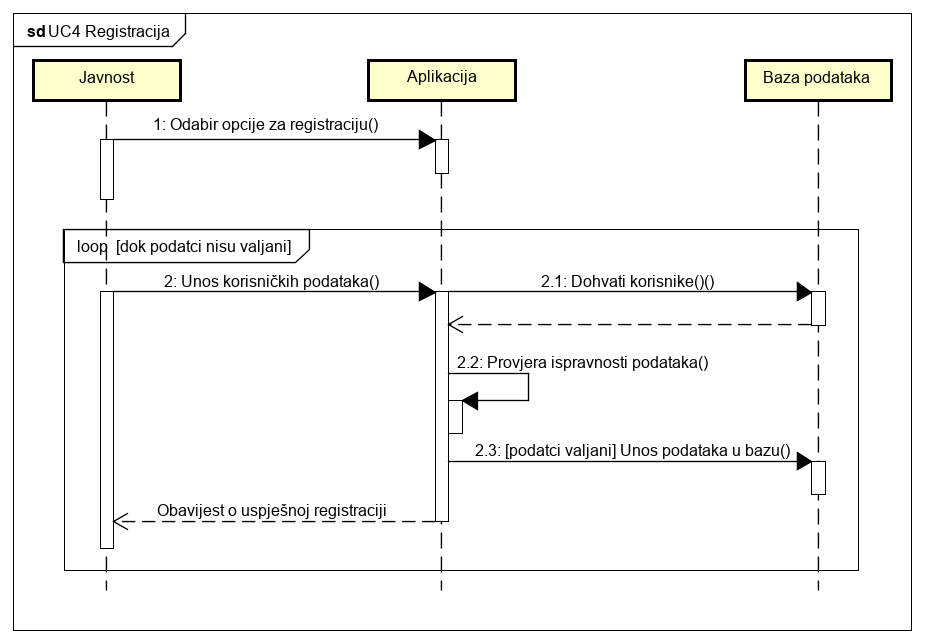
\includegraphics[width=15cm]{slike/UC4.PNG}
					\end{center}
					\caption{Sekvencijski dijagram za UC4}
					\label{fig:uc4}
				\end{figure}
			
				\begin{figure}[H]
					\begin{center}
						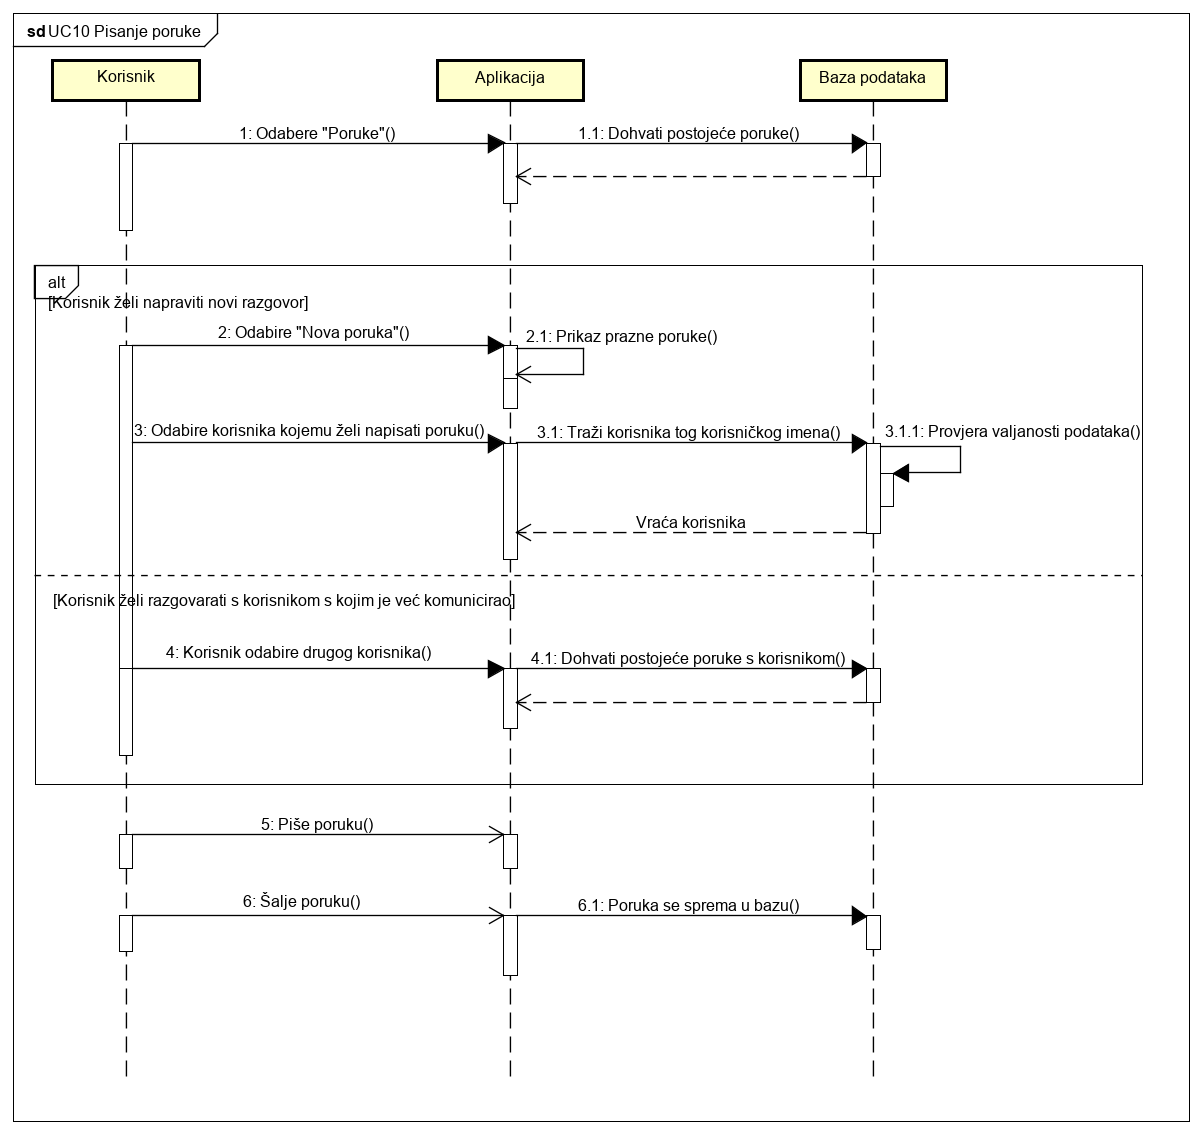
\includegraphics[width=15cm]{slike/UC10.PNG}
					\end{center}
					\caption{Sekvencijski dijagram za UC10}
					\label{fig:uc10}
				\end{figure}
				
				\begin{figure}[H]
					\begin{center}
						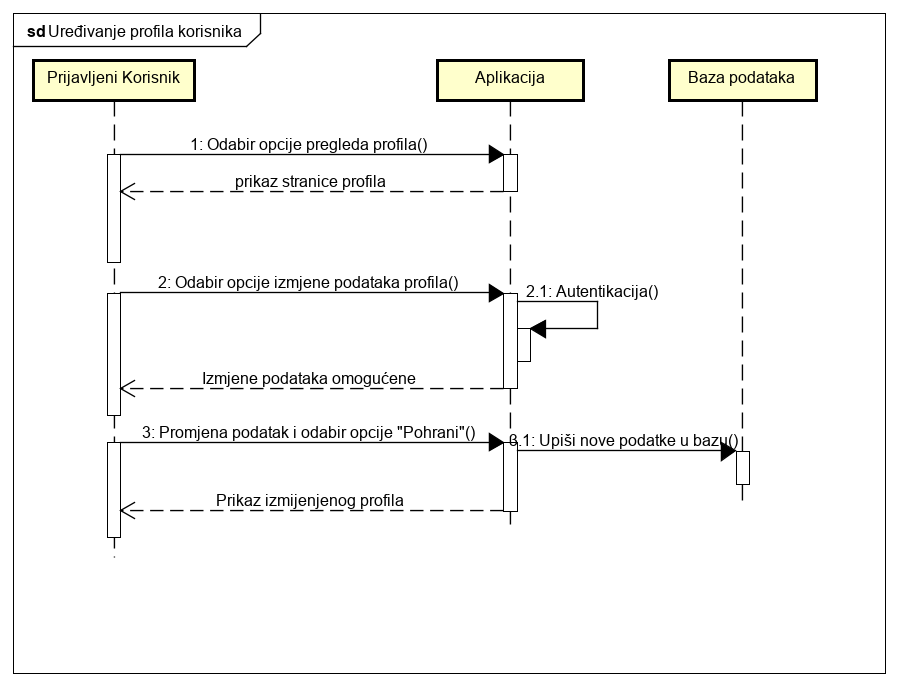
\includegraphics[width=15cm]{slike/uc15.PNG}
					\end{center}
					\caption{Sekvencijski dijagram za UC15}
					\label{fig:uc15}
				\end{figure}
			
			\begin{figure}[H]
				\begin{center}
					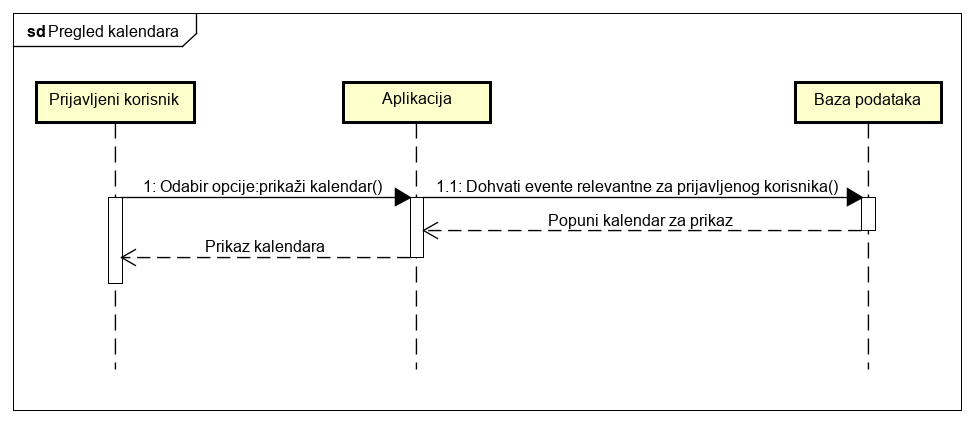
\includegraphics[width=15cm]{slike/uc25.PNG}
				\end{center}
				\caption{Sekvencijski dijagram za UC25}
				\label{fig:uc25}
			\end{figure}
	
		\section{Ostali zahtjevi}
		
			\textbf{\textit{dio 1. revizije}}\\
		 
			 \textit{Nefunkcionalni zahtjevi i zahtjevi domene primjene dopunjuju funkcionalne zahtjeve. Oni opisuju \textbf{kako se sustav treba ponašati} i koja \textbf{ograničenja} treba poštivati (performanse, korisničko iskustvo, pouzdanost, standardi kvalitete, sigurnost...). Primjeri takvih zahtjeva u Vašem projektu mogu biti: podržani jezici korisničkog sučelja, vrijeme odziva, najveći mogući podržani broj korisnika, podržane web/mobilne platforme, razina zaštite (protokoli komunikacije, kriptiranje...)... Svaki takav zahtjev potrebno je navesti u jednoj ili dvije rečenice.}
			 \begin{itemize}
			 	\item  Sustav treba omogućiti rad više korisnika u isto vrijeme
			 	\item  Neispravno korištenje sučelja ne smije na bilo koji način promijeniti ili obustaviti rad sustava
			 	\item  Sustav mora biti jednostavan za uporabu, tj. mora biti intuitivan
			 	\item Aplikacija mora podržavati hrvatske dijakritične znakove
			 	\item  Sustav mora biti u stanju brzo obraditi dobivene podatke kako korisnik ne bi puno čekao promjenu
			 	\item  Sustav treba biti implementiran kao web aplikacija, s time da bi joj većina korisnika pristupala preko mobilnih uređaja
			 	\item Web aplikacija treba biti implementirana koristeći objektno-orijentirane jezike
			 	\item  Treba osigurati sigurnost aplikacije, tj. lozinke moraju biti enkriptirane te mora biti osigurana sigurnost veze između korisnika aplikacije i baze podataka 
			 \end{itemize}
			 
			 
	